\documentclass{beamer}
\usepackage{listings}
\lstset{
%language=C,
frame=single, 
breaklines=true,
columns=fullflexible
}
\usepackage{subcaption}
\usepackage{url}
\usepackage{tikz}
\usepackage{tkz-euclide} % loads  TikZ and tkz-base
%\usetkzobj{all}
\usetikzlibrary{calc,math}
\usepackage{float}
\newcommand\norm[1]{\left\lVert#1\right\rVert}
\providecommand{\pr}[1]{\ensuremath{\Pr\left(#1\right)}}
\renewcommand{\vec}[1]{\mathbf{#1}}
\usepackage[export]{adjustbox}
\usepackage[utf8]{inputenc}
\usepackage{amsmath}
\usetheme{Boadilla}

\title{GATE EC 2017- Q.7}
\author{Tanmay Goyal - AI20BTECH11021}

\date{}

\begin{document}

\begin{frame}
\titlepage
\end{frame}
\begin{frame}
\frametitle{Question}
\begin{flushleft}
The input $x(t)$ and output $y(t)$ of a continous time signal are related as:
\begin{align}
    y(t) = \int_{t-T}^tx(u)\,du
\end{align}
The system is:
\begin{enumerate}
    \item Linear and Time-variant
    \item Linear and Time-invariant
    \item Non-Linear and Time-variant
    \item Non-Linear and Time-invariant
\end{enumerate}
\end{flushleft}
\end{frame}

\begin{frame}[fragile]
\frametitle{Linear Systems and Time Invariant Systems}

\begin{flushleft}
\begin{definition}
We say that a system is\textbf{ linear} if and only if it follows the Principle of Superposition, i.e Law of Additivity and Law of Homogeneity.
\label{L}
\end{definition}
          \end{flushleft}
    \begin{flushleft}
    \begin{definition}
A system is said to be \textbf{time invariant} if the output signal does not depend on the absolute time, i.e a time delay on the input signal directly equates to the delay in the output signal.
\label{T}
\end{definition}
\end{flushleft}
\end{frame}


\begin{frame}[fragile]
\frametitle{Lemma}
\begin{flushleft}
\begin{lemma}
The system relating the input signal $x(t$) and output signal $y(t)$, given by 
\begin{align}
     y(t) = \int_{t-T}^tx(u)\,du
\end{align}
is linear and time invariant in nature.
\end{lemma}
\end{flushleft}

\end{frame}

\begin{frame}{fragile}
\frametitle{Proof: Law of Additivity}

\begin{flushleft}
Let the input signals be $x_1(t)$ and $x_2(t)$, and their corresponding output signals be $y_1(t)$ and $y_2(t)$, then:
\begin{align}
    y_1(t) = \int_{t-T}^tx_1(u)\,du\\
    y_2(t) = \int_{t-T}^tx_2(u)\,du\\
    y_1(t) + y_2(t) = \int_{t-T}^t[x_1(u) + x_2(u)]\,du
    \label{1}
\end{align}
\end{flushleft}

\end{frame}
\begin{frame}{fragile}
\frametitle{Proof: Law of Additivity}

\begin{flushleft}
Now, consider the input signal of $x_1(t) + x_2(t)$, then the corresponding output signal is given by $y'(t)$:
\begin{align}
    y'(t) = \int_{t-T}^t[x_1(u) + x_2(u)]\,du
    \label{2}
\end{align}
Clearly, from \eqref{1} and \eqref{2}:
\begin{align}
    y'(t) = y_1(t) + y_2(t)
\end{align}
Thus, the Law of Additivity holds.\\

\end{flushleft}
    
\end{frame}

\begin{frame}
    \frametitle{Proof: Law of Homogeneity}
    \begin{flushleft}
      Consider an input signal $kx(t)$, where $k$ is any constant. Let the corresponding output be given by $y'(t)$, then:
\begin{align}
    y'(t) = \int_{t-T}^t kx(u)\,du\\
    = k\int_{t-T}^t x(u)\,du\\
     = ky(t)
     \label{3}
\end{align}
Clearly, from \eqref{3},
\begin{align}
    y'(t) = ky(t)
\end{align}
Thus, the Law of Homogeneity holds.\\
  \end{flushleft}
\end{frame}

\begin{frame}
    \frametitle{Proof}
    \begin{flushleft}
    Since both the Laws hold, the system satisfies the Principle of Superposition, and is thus, a \textbf{linear system}.\\
    \end{flushleft}
\end{frame}

\begin{frame}
    \frametitle{Proof: Time Invariance}
    \begin{flushleft}
    To check for time-invariance, we would introduce a delay of $t_0$ in the output and input signals.\\
Delay in output signal:
\begin{align}
    y(t-t_0) = \int_{t-t_0-T}^{t-t_0} x(u)\,du
    \label{4}
\end{align}
    \end{flushleft}
\end{frame}

\begin{frame}
    \frametitle{Proof: Time Invariance}
    \begin{flushleft}
    Now, we consider an input signal with a delay of $t_0$, given by $x(t-t_0)$, and let the corresponding output signal be given by $y'(t)$, then:
\begin{align}
    y'(t) = \int_{t-T}^{t} x(u-t_0)\,du
\end{align}
Substituting $a = u-t_0$:
\begin{align}
    y'(t) = \int_{t-t_0-T}^{t-t_0} x(a)\,da
    \label{5}
\end{align}
Clearly, from \eqref{4} and \eqref{5}:
\begin{align}
    y'(t) = y(t-t_0)
\end{align}
Thus, the system is \textbf{time-invariant}.\\

 Thus, \textbf{2) Linear and Time- invariant} is the correct answer.
    \end{flushleft}
\end{frame}

\begin{frame}
    \frametitle{Impulse response}
    \begin{flushleft}
    Since the given system is an LTI system, it would possess an impulse response $h(t)$, which is the output of the system when the input signal is the Impulse function, given by $\delta(t)$. Thus,
\begin{align}
    h(t) = \int_{t-T}^{t} \delta(u)du
\end{align}
    \end{flushleft}
\end{frame}
\begin{frame}
    \frametitle{Impulse function}
    \begin{flushleft}
    The Impulse function can be loosely defined as:
\begin{align}
    \delta(t) = 
    \begin{cases}
\infty & t = 0\\
0 & otherwise
\end{cases}
and \int_{-\infty}^\infty \delta(t)dt  = 1
\end{align}
    \end{flushleft}
\end{frame}
\begin{frame}
    \frametitle {Impulse response}
    \begin{flushleft}
    Since the Impulse function is zero everywhere aside from $t = 0$ , the non-zero value of integration is a result of $\delta(0)$. Thus, we can say $h(t)$ will be non-zero only if the limits of integration would include $t=0$, i.e:
\begin{align}
    h(t) = 
    \begin{cases}
    \int_{t-T}^{t} \delta(u)du & t-T<0 ; t>0\\
    0 & otherwise
    \end{cases}
    \end{align}
    \begin{align}
h(t) = 
    \begin{cases}
    1 & 0<t<T\\
    0 & otherwise
    \end{cases}
\end{align}
    \end{flushleft}
\end{frame}

\begin{frame}
  \frametitle{Graphs: Input and Output signals}
 \begin{columns}
\begin{column}{0.5\textwidth}
\begin{figure}
\begin{flushleft}
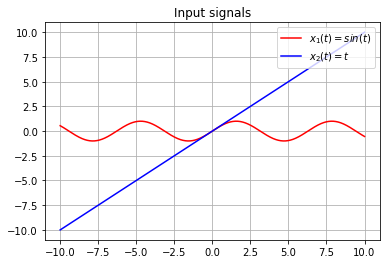
\includegraphics[width=\columnwidth]{graphs/input_signals.png}
 \caption{$x_1(t) = \sin{t}$ and $x_2(t) = t$}
\end{flushleft}
\end{figure}
\end{column}
\begin{column}{0.5\textwidth}
\begin{figure}
\begin{flushleft}
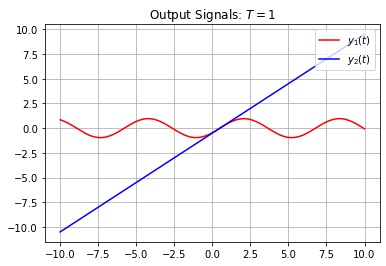
\includegraphics[width=\columnwidth]{graphs/output_signals.png}
 \caption{$y_1(t)$ and  $y_2(t)$}
\end{flushleft}
\end{figure}
\end{column}
\end{columns}
   
   
\end{frame}
\begin{frame}
  \frametitle{Graphs: Laws of Additivity and Homogeneity}
 \begin{columns}
\begin{column}{0.5\textwidth}
\begin{figure}
\begin{flushleft}
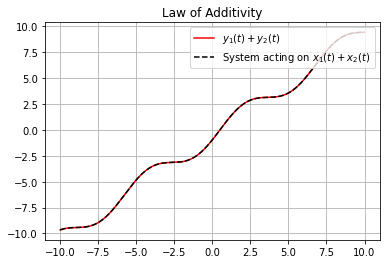
\includegraphics[width=\columnwidth]{graphs/law_of_additivity.png}
 \caption{Law of Additivity}
\end{flushleft}
\end{figure}
\end{column}
\begin{column}{0.5\textwidth}
\begin{figure}
\begin{flushleft}
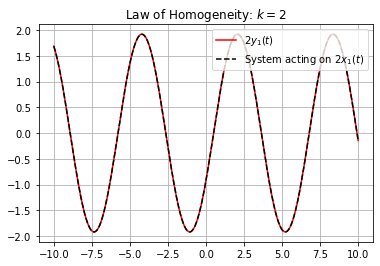
\includegraphics[width=\columnwidth]{graphs/law_of_homogeneity.png}
 \caption{Law of Homogeneity}
\end{flushleft}
\end{figure}
\end{column}
\end{columns}
\end{frame}

\begin{frame}
    \frametitle{Graphs: Time Invariance}
    \begin{figure}
\begin{flushleft}
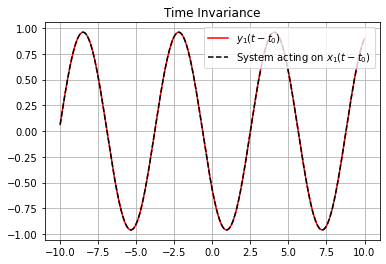
\includegraphics[width=\columnwidth]{graphs/time_invariance.png}

 \caption{Time invariance}
\end{flushleft}
\end{figure}
\end{frame}
\end{document}